\documentclass[twoside]{book}

% Packages required by doxygen
\usepackage{fixltx2e}
\usepackage{calc}
\usepackage{doxygen}
\usepackage[export]{adjustbox} % also loads graphicx
\usepackage{graphicx}
\usepackage[utf8]{inputenc}
\usepackage{makeidx}
\usepackage{multicol}
\usepackage{multirow}
\PassOptionsToPackage{warn}{textcomp}
\usepackage{textcomp}
\usepackage[nointegrals]{wasysym}
\usepackage[table]{xcolor}

% Font selection
\usepackage[T1]{fontenc}
\usepackage[scaled=.90]{helvet}
\usepackage{courier}
\usepackage{amssymb}
\usepackage{sectsty}
\renewcommand{\familydefault}{\sfdefault}
\allsectionsfont{%
  \fontseries{bc}\selectfont%
  \color{darkgray}%
}
\renewcommand{\DoxyLabelFont}{%
  \fontseries{bc}\selectfont%
  \color{darkgray}%
}
\newcommand{\+}{\discretionary{\mbox{\scriptsize$\hookleftarrow$}}{}{}}

% Page & text layout
\usepackage{geometry}
\geometry{%
  a4paper,%
  top=2.5cm,%
  bottom=2.5cm,%
  left=2.5cm,%
  right=2.5cm%
}
\tolerance=750
\hfuzz=15pt
\hbadness=750
\setlength{\emergencystretch}{15pt}
\setlength{\parindent}{0cm}
\setlength{\parskip}{3ex plus 2ex minus 2ex}
\makeatletter
\renewcommand{\paragraph}{%
  \@startsection{paragraph}{4}{0ex}{-1.0ex}{1.0ex}{%
    \normalfont\normalsize\bfseries\SS@parafont%
  }%
}
\renewcommand{\subparagraph}{%
  \@startsection{subparagraph}{5}{0ex}{-1.0ex}{1.0ex}{%
    \normalfont\normalsize\bfseries\SS@subparafont%
  }%
}
\makeatother

% Headers & footers
\usepackage{fancyhdr}
\pagestyle{fancyplain}
\fancyhead[LE]{\fancyplain{}{\bfseries\thepage}}
\fancyhead[CE]{\fancyplain{}{}}
\fancyhead[RE]{\fancyplain{}{\bfseries\leftmark}}
\fancyhead[LO]{\fancyplain{}{\bfseries\rightmark}}
\fancyhead[CO]{\fancyplain{}{}}
\fancyhead[RO]{\fancyplain{}{\bfseries\thepage}}
\fancyfoot[LE]{\fancyplain{}{}}
\fancyfoot[CE]{\fancyplain{}{}}
\fancyfoot[RE]{\fancyplain{}{\bfseries\scriptsize Generated by Doxygen }}
\fancyfoot[LO]{\fancyplain{}{\bfseries\scriptsize Generated by Doxygen }}
\fancyfoot[CO]{\fancyplain{}{}}
\fancyfoot[RO]{\fancyplain{}{}}
\renewcommand{\footrulewidth}{0.4pt}
\renewcommand{\chaptermark}[1]{%
  \markboth{#1}{}%
}
\renewcommand{\sectionmark}[1]{%
  \markright{\thesection\ #1}%
}

% Indices & bibliography
\usepackage{natbib}
\usepackage[titles]{tocloft}
\setcounter{tocdepth}{3}
\setcounter{secnumdepth}{5}
\makeindex

% Hyperlinks (required, but should be loaded last)
\usepackage{ifpdf}
\ifpdf
  \usepackage[pdftex,pagebackref=true]{hyperref}
\else
  \usepackage[ps2pdf,pagebackref=true]{hyperref}
\fi
\hypersetup{%
  colorlinks=true,%
  linkcolor=blue,%
  citecolor=blue,%
  unicode%
}

% Custom commands
\newcommand{\clearemptydoublepage}{%
  \newpage{\pagestyle{empty}\cleardoublepage}%
}

\usepackage{caption}
\captionsetup{labelsep=space,justification=centering,font={bf},singlelinecheck=off,skip=4pt,position=top}

%===== C O N T E N T S =====

\begin{document}

% Titlepage & ToC
\hypersetup{pageanchor=false,
             bookmarksnumbered=true,
             pdfencoding=unicode
            }
\pagenumbering{alph}
\begin{titlepage}
\vspace*{7cm}
\begin{center}%
{\Large My Project }\\
\vspace*{1cm}
{\large Generated by Doxygen 1.8.13}\\
\end{center}
\end{titlepage}
\clearemptydoublepage
\pagenumbering{roman}
\tableofcontents
\clearemptydoublepage
\pagenumbering{arabic}
\hypersetup{pageanchor=true}

%--- Begin generated contents ---
\chapter{Hierarchical Index}
\section{Class Hierarchy}
This inheritance list is sorted roughly, but not completely, alphabetically\+:\begin{DoxyCompactList}
\item K\+Medoids\begin{DoxyCompactList}
\item \contentsline{section}{K\+Meds\+Wrapper}{\pageref{classKMedsWrapper}}{}
\end{DoxyCompactList}
\end{DoxyCompactList}

\chapter{Class Index}
\doxysection{Class List}
Here are the classes, structs, unions and interfaces with brief descriptions\+:\begin{DoxyCompactList}
\item\contentsline{section}{\mbox{\hyperlink{classkm_1_1BanditPAM}{km\+::\+Bandit\+PAM}} \\*Contains all necessary \mbox{\hyperlink{classkm_1_1BanditPAM}{Bandit\+PAM}} functions }{\pageref{classkm_1_1BanditPAM}}{}
\item\contentsline{section}{\mbox{\hyperlink{classkm_1_1FastPAM1}{km\+::\+Fast\+PAM1}} \\*Class implementation for \mbox{\hyperlink{classkm_1_1FastPAM1}{Fast\+PAM1}} algorithm }{\pageref{classkm_1_1FastPAM1}}{}
\item\contentsline{section}{\mbox{\hyperlink{classkm_1_1KMedoids}{km\+::\+KMedoids}} \\*Class implementation for running \mbox{\hyperlink{classkm_1_1KMedoids}{KMedoids}} methods }{\pageref{classkm_1_1KMedoids}}{}
\item\contentsline{section}{\mbox{\hyperlink{classkm_1_1KMedoidsWrapper}{km\+::\+KMedoids\+Wrapper}} \\*Python wrapper for \mbox{\hyperlink{classkm_1_1KMedoids}{KMedoids}} class }{\pageref{classkm_1_1KMedoidsWrapper}}{}
\item\contentsline{section}{\mbox{\hyperlink{classkm_1_1PAM}{km\+::\+PAM}} \\*Class implementation for \mbox{\hyperlink{classkm_1_1PAM}{PAM}} algorithm }{\pageref{classkm_1_1PAM}}{}
\end{DoxyCompactList}

\chapter{File Index}
\section{File List}
Here is a list of all documented files with brief descriptions\+:\begin{DoxyCompactList}
\item\contentsline{section}{/home/esfrankel/\+Desktop/\+Bandit\+P\+A\+M/src/\hyperlink{kmedoids__ucb_8cpp}{kmedoids\+\_\+ucb.\+cpp} }{\pageref{kmedoids__ucb_8cpp}}{}
\item\contentsline{section}{/home/esfrankel/\+Desktop/\+Bandit\+P\+A\+M/src/\hyperlink{kmeds__pywrapper_8cpp}{kmeds\+\_\+pywrapper.\+cpp} }{\pageref{kmeds__pywrapper_8cpp}}{}
\item\contentsline{section}{/home/esfrankel/\+Desktop/\+Bandit\+P\+A\+M/src/\hyperlink{main_8cpp}{main.\+cpp} }{\pageref{main_8cpp}}{}
\end{DoxyCompactList}

\chapter{Class Documentation}
\hypertarget{classKMedsWrapper}{}\section{K\+Meds\+Wrapper Class Reference}
\label{classKMedsWrapper}\index{K\+Meds\+Wrapper@{K\+Meds\+Wrapper}}


Inheritance diagram for K\+Meds\+Wrapper\+:\nopagebreak
\begin{figure}[H]
\begin{center}
\leavevmode
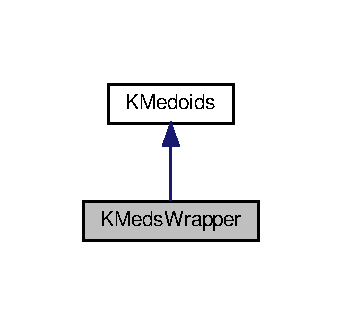
\includegraphics[width=164pt]{classKMedsWrapper__inherit__graph}
\end{center}
\end{figure}


Collaboration diagram for K\+Meds\+Wrapper\+:\nopagebreak
\begin{figure}[H]
\begin{center}
\leavevmode
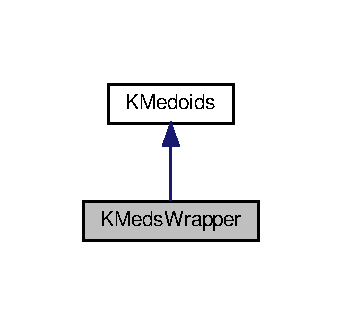
\includegraphics[width=164pt]{classKMedsWrapper__coll__graph}
\end{center}
\end{figure}
\subsection*{Public Member Functions}
\begin{DoxyCompactItemize}
\item 
void \hyperlink{classKMedsWrapper_ac0311bd5d2aef638cf794e4412426d3c}{fit\+Python} (py\+::array\+\_\+t$<$ double $>$ input\+\_\+data, std\+::string loss, int k, std\+::string log\+Filename)
\item 
py\+::array\+\_\+t$<$ double $>$ \hyperlink{classKMedsWrapper_ae825241c43b8bf92912eb59cd12ae1c5}{get\+Medoids\+Final\+Python} ()
\item 
py\+::array\+\_\+t$<$ double $>$ \hyperlink{classKMedsWrapper_af272debff6f3b31490d20b8dc7bec322}{get\+Medoids\+Build\+Python} ()
\item 
py\+::array\+\_\+t$<$ double $>$ \hyperlink{classKMedsWrapper_aba0a92e75230b7853fd533657ead656e}{get\+Labels\+Python} ()
\item 
int \hyperlink{classKMedsWrapper_a25ac2830354eeae7963cdec34d0137e8}{get\+Steps\+Python} ()
\end{DoxyCompactItemize}
\subsection*{Additional Inherited Members}


\subsection{Detailed Description}
\hyperlink{classKMedsWrapper}{K\+Meds\+Wrapper} class. Is the Python wrapper generated by Pybind that allows for calling the C++ code in Python3. 

\subsection{Member Function Documentation}
\mbox{\Hypertarget{classKMedsWrapper_ac0311bd5d2aef638cf794e4412426d3c}\label{classKMedsWrapper_ac0311bd5d2aef638cf794e4412426d3c}} 
\index{K\+Meds\+Wrapper@{K\+Meds\+Wrapper}!fit\+Python@{fit\+Python}}
\index{fit\+Python@{fit\+Python}!K\+Meds\+Wrapper@{K\+Meds\+Wrapper}}
\subsubsection{\texorpdfstring{fit\+Python()}{fitPython()}}
{\footnotesize\ttfamily void K\+Meds\+Wrapper\+::fit\+Python (\begin{DoxyParamCaption}\item[{py\+::array\+\_\+t$<$ double $>$}]{input\+\_\+data,  }\item[{std\+::string}]{loss,  }\item[{int}]{k,  }\item[{std\+::string}]{log\+Filename }\end{DoxyParamCaption})\hspace{0.3cm}{\ttfamily [inline]}}

This is the main function of the \hyperlink{classKMedoids}{K\+Medoids} module\+: this finds the build and swap medoids for the desired data


\begin{DoxyParams}{Parameters}
{\em input\+\_\+data} & Input data to find the medoids of \\
\hline
{\em loss} & The loss function used during medoid computation \\
\hline
{\em k} & The number of medoids to compute \\
\hline
{\em log\+Filename} & The name of the outputted log file \\
\hline
\end{DoxyParams}
\mbox{\Hypertarget{classKMedsWrapper_aba0a92e75230b7853fd533657ead656e}\label{classKMedsWrapper_aba0a92e75230b7853fd533657ead656e}} 
\index{K\+Meds\+Wrapper@{K\+Meds\+Wrapper}!get\+Labels\+Python@{get\+Labels\+Python}}
\index{get\+Labels\+Python@{get\+Labels\+Python}!K\+Meds\+Wrapper@{K\+Meds\+Wrapper}}
\subsubsection{\texorpdfstring{get\+Labels\+Python()}{getLabelsPython()}}
{\footnotesize\ttfamily py\+::array\+\_\+t$<$double$>$ K\+Meds\+Wrapper\+::get\+Labels\+Python (\begin{DoxyParamCaption}{ }\end{DoxyParamCaption})\hspace{0.3cm}{\ttfamily [inline]}}

This function returns the labels/medoids assignments for each datapoint after the final medoids are identified. \mbox{\Hypertarget{classKMedsWrapper_af272debff6f3b31490d20b8dc7bec322}\label{classKMedsWrapper_af272debff6f3b31490d20b8dc7bec322}} 
\index{K\+Meds\+Wrapper@{K\+Meds\+Wrapper}!get\+Medoids\+Build\+Python@{get\+Medoids\+Build\+Python}}
\index{get\+Medoids\+Build\+Python@{get\+Medoids\+Build\+Python}!K\+Meds\+Wrapper@{K\+Meds\+Wrapper}}
\subsubsection{\texorpdfstring{get\+Medoids\+Build\+Python()}{getMedoidsBuildPython()}}
{\footnotesize\ttfamily py\+::array\+\_\+t$<$double$>$ K\+Meds\+Wrapper\+::get\+Medoids\+Build\+Python (\begin{DoxyParamCaption}{ }\end{DoxyParamCaption})\hspace{0.3cm}{\ttfamily [inline]}}

This function returns the build medoids for a \hyperlink{classKMedoids}{K\+Medoids} object. \mbox{\Hypertarget{classKMedsWrapper_ae825241c43b8bf92912eb59cd12ae1c5}\label{classKMedsWrapper_ae825241c43b8bf92912eb59cd12ae1c5}} 
\index{K\+Meds\+Wrapper@{K\+Meds\+Wrapper}!get\+Medoids\+Final\+Python@{get\+Medoids\+Final\+Python}}
\index{get\+Medoids\+Final\+Python@{get\+Medoids\+Final\+Python}!K\+Meds\+Wrapper@{K\+Meds\+Wrapper}}
\subsubsection{\texorpdfstring{get\+Medoids\+Final\+Python()}{getMedoidsFinalPython()}}
{\footnotesize\ttfamily py\+::array\+\_\+t$<$double$>$ K\+Meds\+Wrapper\+::get\+Medoids\+Final\+Python (\begin{DoxyParamCaption}{ }\end{DoxyParamCaption})\hspace{0.3cm}{\ttfamily [inline]}}

This function returns the final medoids for a \hyperlink{classKMedoids}{K\+Medoids} object. \mbox{\Hypertarget{classKMedsWrapper_a25ac2830354eeae7963cdec34d0137e8}\label{classKMedsWrapper_a25ac2830354eeae7963cdec34d0137e8}} 
\index{K\+Meds\+Wrapper@{K\+Meds\+Wrapper}!get\+Steps\+Python@{get\+Steps\+Python}}
\index{get\+Steps\+Python@{get\+Steps\+Python}!K\+Meds\+Wrapper@{K\+Meds\+Wrapper}}
\subsubsection{\texorpdfstring{get\+Steps\+Python()}{getStepsPython()}}
{\footnotesize\ttfamily int K\+Meds\+Wrapper\+::get\+Steps\+Python (\begin{DoxyParamCaption}{ }\end{DoxyParamCaption})\hspace{0.3cm}{\ttfamily [inline]}}

This function returns the number of swap steps that took place during the computation 

The documentation for this class was generated from the following file\+:\begin{DoxyCompactItemize}
\item 
/home/esfrankel/\+Desktop/\+Bandit\+P\+A\+M/src/\hyperlink{kmeds__pywrapper_8cpp}{kmeds\+\_\+pywrapper.\+cpp}\end{DoxyCompactItemize}

\chapter{File Documentation}
\hypertarget{kmedoids__ucb_8cpp}{}\doxysection{/\+Users/dhavaldangaria/\+Bandit\+PAM/src/kmedoids\+\_\+ucb.cpp File Reference}
\label{kmedoids__ucb_8cpp}\index{/Users/dhavaldangaria/BanditPAM/src/kmedoids\_ucb.cpp@{/Users/dhavaldangaria/BanditPAM/src/kmedoids\_ucb.cpp}}
{\ttfamily \#include \char`\"{}kmedoids\+\_\+ucb.\+hpp\char`\"{}}\newline
{\ttfamily \#include $<$carma.\+h$>$}\newline
{\ttfamily \#include $<$armadillo$>$}\newline
{\ttfamily \#include $<$unordered\+\_\+map$>$}\newline
{\ttfamily \#include $<$regex$>$}\newline
Include dependency graph for kmedoids\+\_\+ucb.\+cpp\+:
\nopagebreak
\begin{figure}[H]
\begin{center}
\leavevmode
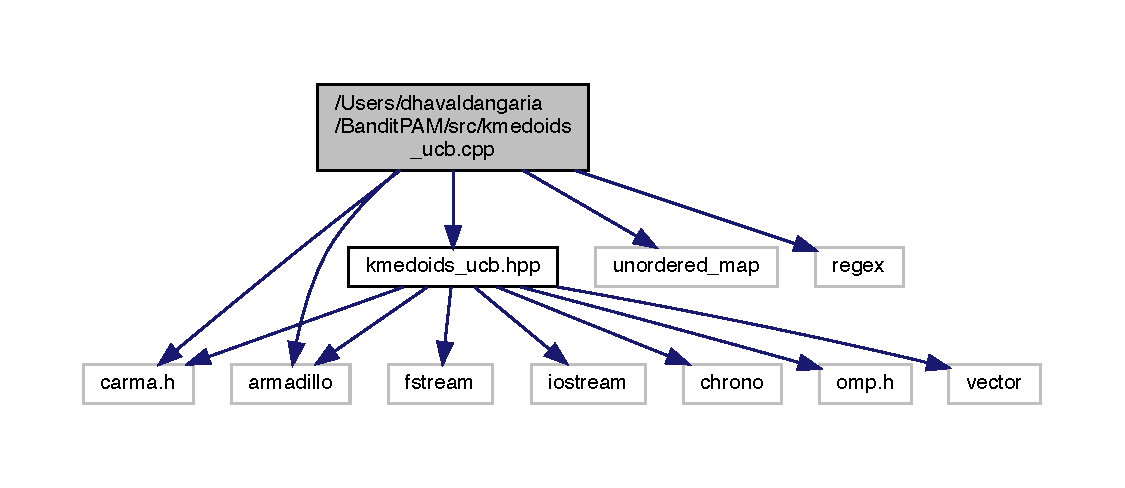
\includegraphics[width=350pt]{kmedoids__ucb_8cpp__incl}
\end{center}
\end{figure}


\doxysubsection{Detailed Description}
\begin{DoxyDate}{Date}
2020-\/06-\/10
\end{DoxyDate}
This file contains the primary C++ implementation of the Bandit\+PAM code. 

\hypertarget{kmeds__pywrapper_8cpp}{}\section{/home/esfrankel/\+Desktop/\+Bandit\+P\+A\+M/src/kmeds\+\_\+pywrapper.cpp File Reference}
\label{kmeds__pywrapper_8cpp}\index{/home/esfrankel/\+Desktop/\+Bandit\+P\+A\+M/src/kmeds\+\_\+pywrapper.\+cpp@{/home/esfrankel/\+Desktop/\+Bandit\+P\+A\+M/src/kmeds\+\_\+pywrapper.\+cpp}}
{\ttfamily \#include $<$armadillo$>$}\newline
{\ttfamily \#include $<$carma/carma.\+h$>$}\newline
{\ttfamily \#include $<$pybind11/pybind11.\+h$>$}\newline
{\ttfamily \#include $<$pybind11/numpy.\+h$>$}\newline
{\ttfamily \#include \char`\"{}kmedoids\+\_\+ucb.\+hpp\char`\"{}}\newline
Include dependency graph for kmeds\+\_\+pywrapper.\+cpp\+:\nopagebreak
\begin{figure}[H]
\begin{center}
\leavevmode
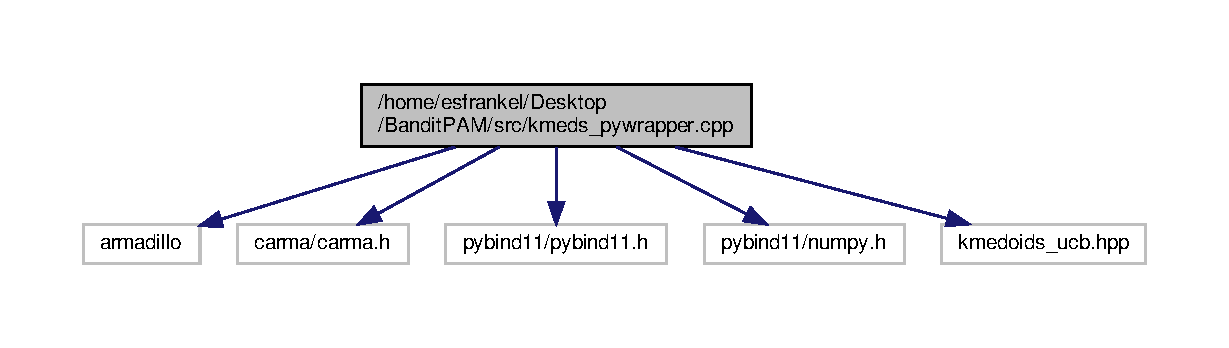
\includegraphics[width=350pt]{kmeds__pywrapper_8cpp__incl}
\end{center}
\end{figure}
\subsection*{Classes}
\begin{DoxyCompactItemize}
\item 
class \hyperlink{classKMedsWrapper}{K\+Meds\+Wrapper}
\begin{DoxyCompactList}\small\item\em Python wrapper for \hyperlink{classKMedoids}{K\+Medoids} class. \end{DoxyCompactList}\end{DoxyCompactItemize}
\subsection*{Functions}
\begin{DoxyCompactItemize}
\item 
\mbox{\Hypertarget{kmeds__pywrapper_8cpp_a66c5e3323d71e29a0a148bec731ac27b}\label{kmeds__pywrapper_8cpp_a66c5e3323d71e29a0a148bec731ac27b}} 
{\bfseries P\+Y\+B\+I\+N\+D11\+\_\+\+M\+O\+D\+U\+LE} (Bandit\+P\+AM, m)
\end{DoxyCompactItemize}


\subsection{Detailed Description}
\begin{DoxyDate}{Date}
2020-\/06-\/10
\end{DoxyDate}
Creates the Python bindings for the C++ code that allows it to be called in Python. 
\hypertarget{main_8cpp}{}\doxysection{/\+Users/motiwari/\+Desktop/\+Bandit\+PAM/src/main.cpp File Reference}
\label{main_8cpp}\index{/Users/motiwari/Desktop/BanditPAM/src/main.cpp@{/Users/motiwari/Desktop/BanditPAM/src/main.cpp}}
{\ttfamily \#include \char`\"{}kmedoids\+\_\+algorithm.\+hpp\char`\"{}}\newline
{\ttfamily \#include $<$armadillo$>$}\newline
{\ttfamily \#include $<$chrono$>$}\newline
{\ttfamily \#include $<$fstream$>$}\newline
{\ttfamily \#include $<$unistd.\+h$>$}\newline
{\ttfamily \#include $<$exception$>$}\newline
{\ttfamily \#include $<$regex$>$}\newline
{\ttfamily \#include $<$filesystem$>$}\newline
Include dependency graph for main.\+cpp\+:
\nopagebreak
\begin{figure}[H]
\begin{center}
\leavevmode
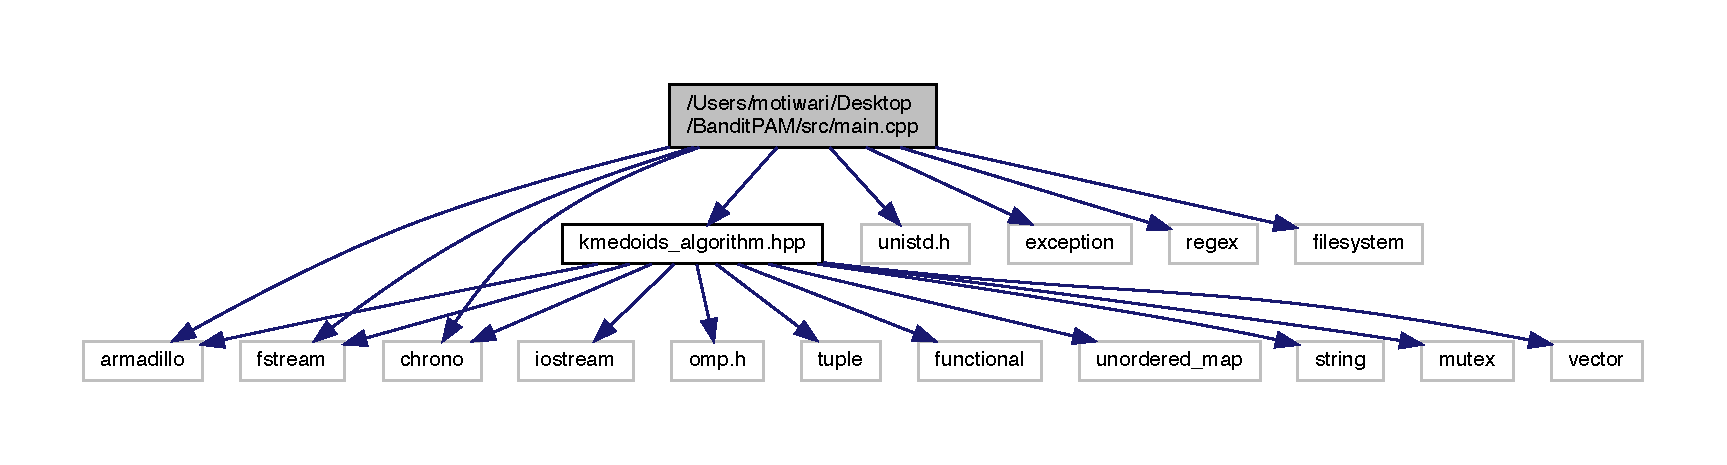
\includegraphics[width=350pt]{main_8cpp__incl}
\end{center}
\end{figure}
\doxysubsection*{Functions}
\begin{DoxyCompactItemize}
\item 
\mbox{\Hypertarget{main_8cpp_a0ddf1224851353fc92bfbff6f499fa97}\label{main_8cpp_a0ddf1224851353fc92bfbff6f499fa97}} 
int {\bfseries main} (int argc, char $\ast$argv\mbox{[}$\,$\mbox{]})
\end{DoxyCompactItemize}


\doxysubsection{Detailed Description}
\begin{DoxyDate}{Date}
2020-\/06-\/10
\end{DoxyDate}
Defines a command line program that can be used to run the \mbox{\hyperlink{classBanditPAM}{Bandit\+PAM}} KMedoids algorithm.

Usage (from home repo directory)\+: ./src/build/\+Bandit\+PAM -\/f \mbox{[}path/to/input\mbox{]} -\/k \mbox{[}number of clusters\mbox{]} 

%--- End generated contents ---

% Index
\backmatter
\newpage
\phantomsection
\clearemptydoublepage
\addcontentsline{toc}{chapter}{Index}
\printindex

\end{document}
